\title{Year 12 Chemistry Depth Study}
\author{
NESA \#: 34364338 
}

\documentclass[12pt, a4paper]{article}
\usepackage[margin=0.5in]{geometry}
\usepackage{parskip}
\usepackage{amsmath}
\usepackage{float}
\usepackage[T1]{fontenc}

\usepackage{graphicx}
\graphicspath{ {./images/} }

\begin{document}
\maketitle





\section{Equilibrium Systems: Contact Process}

The Contact Process is a multi-step industrial process used to produce concentrated sulfuric acid. 

\begin{enumerate}
	\item Produce sulfur dioxide from sulfur and excess oxygen
	\item Convert sulfur dioxide to sulfur trioxide
	\item Produce oleum (fuming sulfuric acid) from sulfur trioxide
	\item React oleum with water to produce concentrated sulfuric acid
\end{enumerate}






\subsection{Exploring the Contact Process}

\subsubsection{Producing sulfur dioxide}

To produce sulfur dioxide, an irreversible exothermic combustion reaction between sulfur and oxygen is used to produce sulfur dioxide.

\begin{align}
	S(s) + O_{2}(g) \rightarrow SO_{2}(g)
\end{align}

\subsubsection{Sulfur dioxide to sulfur trioxide}

The conversion of sulfur dioxide to sulfur trioxide is an exothermic reversible reaction, generally performed in a contact tower or oxidation chamber.

\begin{align}
	2SO_{2}(g) + O_{2} \rightleftharpoons 2SO_{3}(g) \qquad \qquad \Delta H = -196 \; kJ \; mol^{-1}
\end{align}

\pagebreak






\subsubsection{Producing concentrated sulfuric acid}

After the production of sulfur trioxide, sulfuric acid is produced in an absorption tower. For a more stable reaction, sulfur trioxide is first dissolved in concentrated sulfuric acid, to produce \textbf{oleum} (or fuming sulfuric acid). Without this initial step, the reaction would produce sulfuric acid gas (as a mist or vapor) as the reaction would be highly exothermic.

\begin{align}
	H_{2}SO_{4}(l) + SO_{3}(g) \rightarrow H_{2}S_{2}O_{7}(l)
\end{align}

Once oleum is produced, it is safely reacted with water to produce concentrated sulfuric acid, in a dilution tank.

\begin{align}
	H_{2}S_{2}O_{7}(l) + H_{2}O(l) \rightarrow 2H_{2}SO_{4}(l)
\end{align}

As indicated by the molar ratio in reactions (3) and (4), the production of concentrated sulfuric acid from oleum produces twice as much concentrated sulfuric acid, as what was originally used to produce oleum.






\subsection{The importance and uses of sulfuric acid}

Sulfuric acid is a key primary product used to produce a number of other chemical compounds, and the Contact Process allows them to be produced efficently in high concentrations at industrial scales. 

\subsubsection{Fertilisers}
Sulfuric acid is a key reactant for the production of phosphate-based fertilisers. For example, calcium phosphates are often used as fertiliser and is produced by reacting phosphorite with sulfuric acid.

\begin{align}
	Ca_{3}(PO_{4})_{2}(s) + H_{2}SO_{4}(aq) \rightarrow Ca(H_{2}PO_{4})_{2}(s) + 2CaSO_{4}(s)
\end{align}

Phosphate-based fertilisers are critical to the world's food supply, in ensuring that there is enough food production to sustain a growing world population. According to researchers, without phosphate and nitrogen-based fertilisers, humanity would only be able to produce half its current food production.\footnote{Faradji \& de Boer, 2016.}

\subsubsection{Cleaning agents}
Outside of fertiliser, sulfuric acid is also used as an industrial cleaning agent. It helps to remove oxidation and rust from iron and steel-based components in the passenger motor vehicles (PMV) and major appliances industries, while also featuring as an ingredient in some household cleaning agents such as drain cleaners.






\subsection{Factors affecting equilibrium}

\textbf{Le Chatelier's Principle} states that within equilibrium, a disturbance caused by changing conditions (such as temperature, pressure and concentration) will result in an \textbf{equilibrium shift} to counteract and re-establish the equilibrium. In the case of the Contact Process, it features one \textbf{equilibrium reaction}: the conversion of sulfur dioxide to sulfur trioxide.

\begin{align}
	2SO_{2}(g) + O_{2} \rightleftharpoons 2SO_{3}(g) \qquad \qquad \Delta H = -196 \; kJ \; mol^{-1}
\end{align}






\subsubsection{Temperature}

The forward reaction is \textbf{exothermic} (\(\Delta H = -196 \; kJ \: mol^{-1}\)). By \textbf{Le Chatelier's Principle}, lowering temperature will favour the exothermic side of the reaction. Hence, as temperature decreases, the equilibrium shifts right and the disturbance of the equilibrium is counteracted by an increase in the production of sulfur trioxide. 

However, as temperature decreases, there is less kinetic energy and less frequent successful collisions, hence the rate of reaction decreases (as increased energy is required to break bonds). Therefore, to produce a reasonably high yield at a fast rate, a higher compromise temperature of 400°C to 450°C is often used in industrial applications. As seen in the provided graph, this temperature will gain 80\% (at 450°C) to 90\% (at 400°C) yield, with minimal yield increases as temperature approaches zero.

\begin{center}
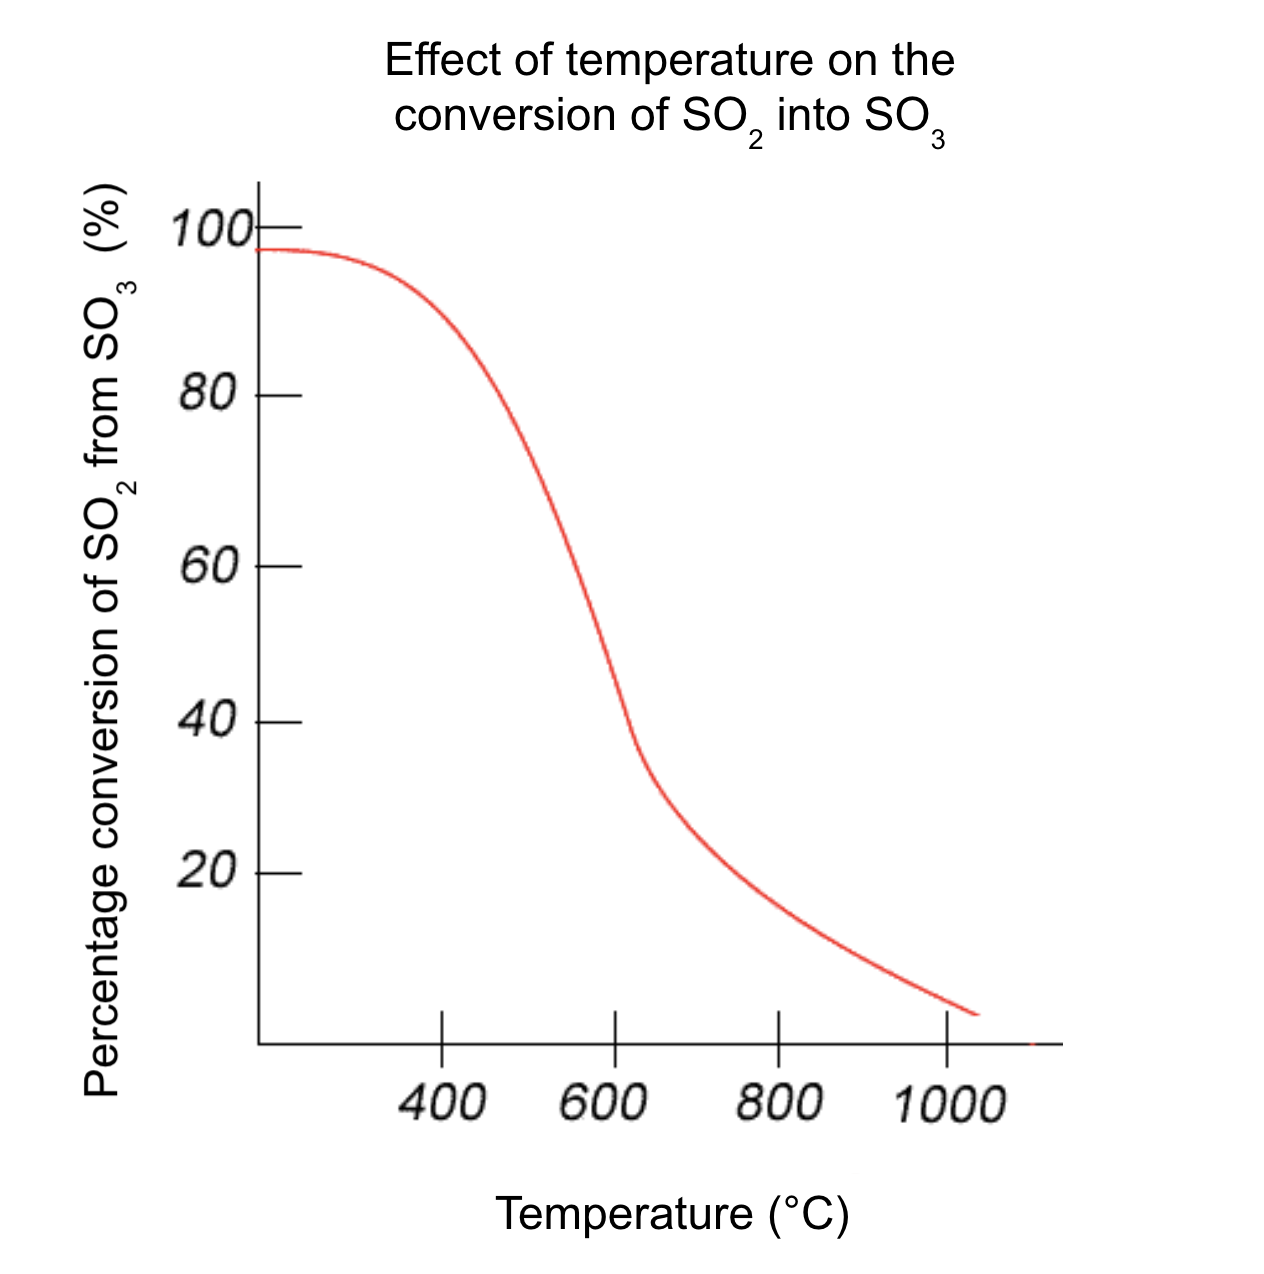
\includegraphics[scale=0.5]{graph}
\\
\textbf{Figure 1:} Temperature/yield graph for the conversion of \(SO_{2}\) into \(SO_{3}\)
\end{center}






\subsubsection{Pressure}

By \textbf{Le Chatelier's Principle}, an increase in pressure will favour the side with fewer number of moles. In this case, this is the products side, and the equilibrium shifts right. The system will then counteract the disturbance by decreasing pressure, both increasing the rate of reaction, as well as producing more sulfur trioxide.

However, low pressure can still garner an extremely high rate of sulfur dioxide to sulfur trioxide. In industrial applications, lower pressures are used, as they still generate high yield (99.5\%) and often it is economically not justifiable to invest in substantially higher pressures for minimal yield gain.






\subsubsection{Concentration}

By \textbf{Le Chatelier's Principle}, an increase in reactants will disturb equilibrium. This will cause increased collisions, and hence an increased rate of the forward reaction. Initially, the rate of the reverse reaction remains unchanged but eventually the two rate of reactions will approach equilibrium and become constant once more, causing a shift to the right and producing more sulfur trioxide. 






\subsubsection{Catalyst}

\textbf{Catalysts} lower the activation energy required for the reaction to take place, increasing the rate of reaction. By lowering the activation energy, the bonds in the reactants weaken, thereby increasing the rate of reaction, and eliminating the need for otherwise-needed expensive high-pressure systems.

Within the equilibrium reaction, a catalyst of vanadium(V) oxide (\(V_{2}O_{5}\)) is used for a reversible reaction, enabling a dynamic equilibrium to be established. Without a catalyst, the reaction would virtually remain at a static equilibrium.






\section{Industrial Design: Solvay Process}

The Solvay Process is a synthesis reaction which reacts carbon dioxide (produced from limestone), ammonia and brine to produce sodium carbonate. 


\subsection{Exploring the Solvay Process}

The process can be illustrated in the following flowchart:

\begin{center}
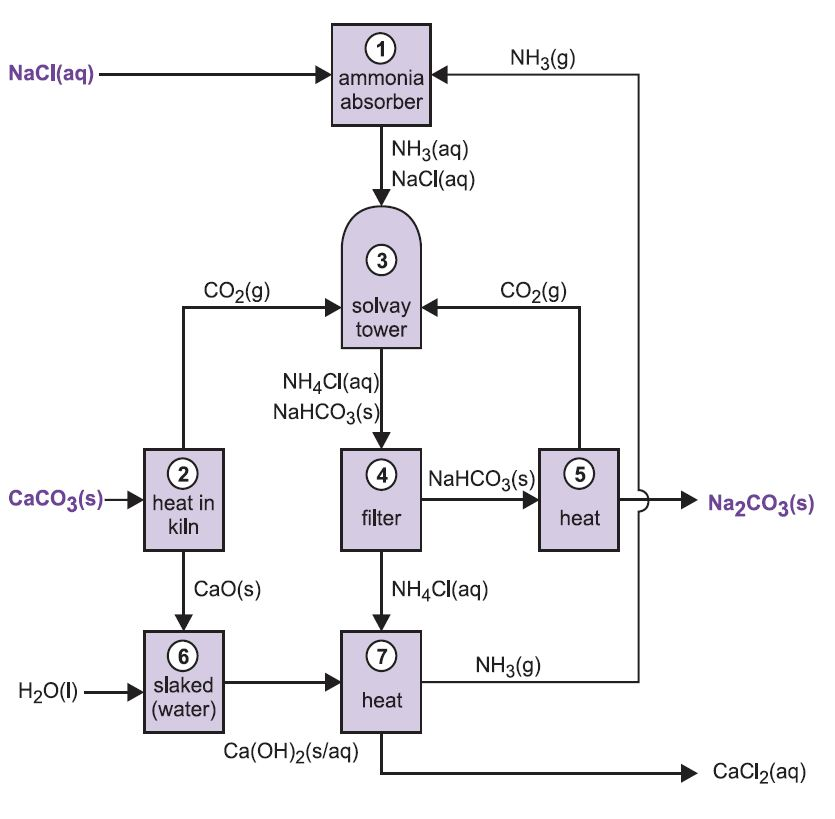
\includegraphics[scale=0.6]{solvay.jpeg}
\\
\textbf{Figure 2:} Flowchart of the Solvay Process
\end{center}




\subsubsection{Ammonia gas as a reactant}

\(NaCl(aq)\) is brine, a highly concentrated and commonly-occuring salt solution which can be sourced underground. When fed through the ammonia absorber at (1),  \(NH_{3}(aq)\) is added to the reactants. \(NH_{3}(aq)\), although expensive to produce (most commonly through the Haber Process), is usually recycled in high proportions during the reaction, which is discussed in a later section


\begin{align}
	Ca(OH)_{2}(s) + 2NH_{4}Cl(aq) \rightarrow 2NH_{3}(g) + CaCl_{2}(aq) + 2H_{2}O(l) \qquad \Delta H = -20 \; kJ \; mol^{-1}
\end{align}


\subsubsection{The effect of heating calcium carbonate}

As part of the Solvay process, large amounts of carbon dioxide gas are needed. This is primarily funded through the calcination of calcium carbonate (limestone) which requires heat. This often takes place in a kiln, depicted at (2), where there is a limestone and coking coal mixture in a 13:1 mass ratio. Coke burns in a counter-current of pre-heated oxygen gas. This process is exothermic and has a negative enthalpy change.

\begin{align}
	C(s) + O_{2}(g) \rightarrow CO_{2}(g) \qquad \Delta H = -65 \; kJ \; mol^{-1}
\end{align}

By combusting coke in an exothermic reaction, this causes the heat of the closed system (kiln) to increase to at least 840°C\footnote{Science Learning Hub, 2021}. Hence, there will be enough energy to establish a dynamic equilibrium for the thermal decomposition of calcium carbonate (an endothermic process with positive enthalpy change).


\paragraph{Producing carbon dioxide}

In order to faciliate the key equilbrium reaction, carbon dioxide must be produced in sufficient quantities. Calcium carbonate is heated at (2) to produce carbon dioxide and calcium oxide, a reversible endothermic process commonly known as \textbf{calcination}. The resulting carbon dioxide can then be used for the Solvay equilibrium reaction.

\begin{align}
	CaCO_{3}(s) + heat \rightleftharpoons CaO(s) + CO_{2}(g) \qquad \qquad \Delta H = +178 \; kJ \; mol^{-1}
\end{align}


\begin{align}
	CaCO_{3}(s) + heat \rightleftharpoons CaO(s) + CO_{2}(g) \qquad \qquad \Delta H = +178 \; kJ \; mol^{-1}
\end{align}


\subsubsection{Solvay tower}

The key equilibrium reaction involves saturating brine (sodium chloride solution) with ammonia gas and carbon dioxide to form ammonium chloride and sodium bicarbonate, which takes place in the Solvay tower at (3) in the flowchart. At low temperatures, the reaction shifts right towards the exothermic products side of the reaction. Sodium bicarbonate crystallises at low temperatures, hence it is solid.

\begin{align}
	NaCl(aq) + NH_{3}(aq) + H_{2}O(l) + CO_{2}(g) \rightleftharpoons NH_{4}Cl(aq) + NaHCO_{3}(s)  \qquad \Delta H = -158 \; kJ \; mol^{-1}
\end{align}


\subsubsection{Filtering sodium bicarbonate}

At (4), aqueous ammonia chloride is filtered from solid sodium bicarbonate. Sodium bicarbonate is heated at (5) to form sodium carbonate, the final product.

\begin{align}
	2NaHCO_{3}(s) + heat \rightleftharpoons Na_{2}CO_{3}(s) + H_{2}O(g) + CO_{2}(g) \qquad \Delta H = +85 \; kJ \; mol^{-1}
\end{align}



\subsubsection{Heating sodium bicarbonate}

Sodium bicarbonate is heated (and hence dehydrated) at (5) in order to produce sodium carbonate, and will begin to thermally decompose at around 100°C, with complete conversion at 200°C\footnote{Senese, 2010}.

\begin{align}
	2NaHCO_{3}(s) + heat \rightleftharpoons Na_{2}CO_{3}(s) + H_{2}O(g) + CO_{2}(g) \qquad \Delta H = +85 \; kJ \; mol^{-1}
\end{align}




\subsubsection{Recycling calcium oxide to form ammonia gas}

In the previous reaction, calcium oxide is also produced alongside carbon dioxide. This can be used to form ammonia gas, an important reactant in the equilibrium reaction. It is first reacted with water to form calcium hydroxide in a process known as \textbf{slaking}, located at (6).

\begin{align}
	CaO(s) + H_{2}O(l) \rightarrow Ca(OH)_{2} \qquad \Delta H = -65 \; kJ \; mol^{-1}
\end{align}

Calcium hydroxide is then reacted and heated with the produced ammonium chloride \(NH_{4}Cl\) from the equilibrium reaction, to form ammonia gas, calcium chloride and water, depicted at (7). Hence, ammonia gas is often recycled through this reaction.



\subsection{Risk assessment}

\begin{table}[H]
	\centering
\begin{tabular}{|p{5cm}|p{12cm}|}
	\hline
\textbf{Risk}                    & \textbf{Hazard}                                                                                                                                                                                                                                                                                                                                                                                                   \\  \hline
Heating of calcium carbonate     & Calcium carbonate is heated at extremely high temperatures of 600-800°C. There is a fire hazard given the presence of flammable material.                                                                                                                                                                                                                                                                        \\  \hline
Ammonia gas                      & Ammonia is flammable, corrosive and highly toxic. If it were to be inhaled, it could cause death, life-threatening pulmonary edema (fluid in the lungs) or breathing difficulties. As it is corrosive, it were to come into contact with skin or eyes, it could irritate or burn, causing scarring on skin or permanent blindness in eyes.                                                                        \\  \hline
Carbon dioxide gas               & Exposure to high concentrations of carbon dioxide gas can lead to drowsiness, headaches, dizziness, increased heart rate, or nausea. At 5000 ppm and above, this could lead to oxygen deprivation.                                                                                                                                                                                                                \\  \hline
Calcium oxide as a waste product & Calcium oxide is an irritant and is corrosive. Contact with the skin or eyes could cause irritation and burning. Inhalation of calcium oxide could cause coughing or breathing difficulties.  In more severe cases, it could cause life-threatening pulmonary edema (fluid in the lungs). Long-term exposure may result in a hole within the inner nose bone. It can cause brittle nails or thicken/cracken skin. \\  \hline
Calcium hydroxide                & Calcium hydroxide is an irritant. It could cause eye damage if it came into contact with eyes.                                                                                                                                                                                                                                                                                                                    \\  \hline
Ammonium chloride                & Ammonium chloride is an irritant and contact with skin could case irritation. Contact with eyes may cause eye damage. Inhaling ammonium chloride fumes may also cause coughing or breathing difficulties.

\\ \hline                                                 

\end{tabular}
\end{table}


\subsection{Assessment of key considerations}

This section assesses the relevant key economical, environmental and social considerations applicable to the Solvay Process at Penrice Factory, Osbourne SA, operational from 1935 to 2014.

\subsubsection{Economical}

Penrice Factory is situated in Osborne, South Australia, around 21 km north-west of the Adelaide city centre, and its location provides many economic and logistical advantages. It is in close proximity to raw materials and environmental features, including the Port River, the St Kilda salt lagoons, and the Penrice limestone quarry in the Barossa Valley. The Perince Stone Train was a limestone train which transported limestone from the quarry to Penrice Factory. Furthermore, its close proximity to the Osborne Power Station allowed it to use steam from the station, making the Penrice Factory the largest cogeneration facility in Australia, which is piped through under the Port River. Being located in Adelaide, it means that there is an expanded local labour market with sufficient housing and public services.

\subsubsection{Environmental}

Penrice Factory has had a number of environmental considerations associated with it. In 2003, the South Australia Environment Protection Authority (EPA) cited Penrice Factory as being one of the main sources of oxidised nitrogen and ammonia being present within the Port River Estuary. Other outflow includes calcium chloride and nitrogen. High nutrient concentrations leads to excessive algae and plant growth (which in term can produce toxins and make shellfish unsafe for human consumption), cause fish deaths, or suffocate seagrass. In response, Penrice Factory built commissioned a settling pond system, which is equipped to remove turbidity from water bodies, completed in April 2001. It reduced the amount of suspended solids by 95\%. Penrice Soda Products (operator of the plant) also committed to a \$1.5 million dredging operation in 2008.According to the EPA's water quality report, Penrice Factory initiated an environment improvement program in order to aim reducing ammonia in wastewater discharge. Furthermore, outflow from the factory is responsible for thermal pollution (the discharge of heated water) of the estuary, given that the Solvay process is largely exothermic. 

However, the Solvay process is considered to be at least a partially green reaction. It recycles ammonia and carbon dioxide, such that only small amounts of ammonia need to be refilled at intervals. Obtaining reactants has minimal environmental impact, given that sodium chloride solution (brine) can be formed from dissolving salt in fresh water, or by pumping naturally-occuring brine from the ground. Limestone is naturally abundant and can be easily obtained with minimal environmental impact.

\subsubsection{Social}

- noise
- jobs

\subsubsection{Justification for location suitability}


\pagebreak

\section{Bibliography}

British Broadcasting Corporation 2021, Sulfuric acid and the contact process, viewed 17 October 2021, \\ \textless{https://www.bbc.co.uk/bitesize/guides/zb7f3k7/revision/1}\textgreater

Canadian Centre for Occupational Health and Safety, Ammonia, viewed 31 October 2021, \\ \textless{https://www.ccohs.ca/oshanswers/chemicals/chem\_profiles/ammonia.html}\textgreater

Clark, Jim 2021, \emph{The Contact Process}, Truro School in Cornwall, viewed 17 October 2021, \\ \textless{https://chem.libretexts.org/@go/page/3838}\textgreater

Department of Agriculture, Water and the Environment 2019, Sulfuric acid, Commonwealth of Australia, viewed 18 October 2021, \textless{http://www.npi.gov.au/resource/sulfuric-acid}\textgreater

Dynamic Science n.d., Sulfuric acid - contact process, viewed 1 November 2021, \textless{http://www.dynamicscience.com.au/tester/solutions1/chemistry/sulfuricacid.html}\textgreater (Figure 1)

Faradji, Charly \& de Boer, Marissa 2016, \emph{How the great phosphorus shortage could leave us all hungry}, The Conversation, viewed 18 October 2021, \\ \textless{https://theconversation.com/how-the-great-phosphorus-shortage-could-leave-us-all-hungry-54432}\textgreater

IB Chemistry Web 2016, Equilibrium: Industrial Processes 2016, viewed 22 October 2021, \\ \textless{https://www.ibchem.com/IB16/07.27.htm}\textgreater

Manahan, S E 2016, \emph{Industrial Chemical Reactions - The Solvay Process}, University of Missouri, viewed 24 October 2021 \\ \textless{https://chem.libretexts.org/@go/page/285417}\textgreater

New Jersey Department of Health 2016, Right to Know Hazardous Substance Fact Sheet: Ammonium Chloride, viewed 31 October 2021, \\ \textless{https://www.nj.gov/health/eoh/rtkweb/documents/fs/0093.pdf}\textgreater

New Jersey Department of Health and Senior Services 2003, Hazardous Substance Fact Sheet: Calcium Oxide, viewed 31 October 2021, \\ \textless{https://nj.gov/health/eoh/rtkweb/documents/fs/0325.pdf}\textgreater

Royal Society of Chemistry n.d., Part 4: Manufacturing sodium carbonate by the Solvay process, viewed 29 October 2021, \\ \textless{https://edu.rsc.org/download?ac=15607}\textgreater

Royal Society of Chemistry n.d., Part 5: The thermodynamics and equilibria involved in the Solvay process for producing sodium carbonate, viewed 29 October 2021, \\ \textless{https://edu.rsc.org/download?ac=15610}\textgreater

Science Learning Hub 2021, Carbonate chemistry, viewed 31 October 2021, \\ \textless{https://www.sciencelearn.org.nz/resources/469-carbonate-chemistry}\textgreater

Senese, Fred 2010, \emph{What happens when sodium bicarbonate is headed?}, General Chemistry Online! (Frostburg State University's Department of Chemistry), \\ \textless{https://antoine.frostburg.edu/chem/senese/101/inorganic/faq/carbonate-decomposition.shtml}\textgreater

The Essential Chemistry Industry 2016, Sulfuric acid, viewed 18 October 2021, \\ \textless{https://www.essentialchemicalindustry.org/chemicals/sulfuric-acid.html}\textgreater

Vedantu, Contact Process n.d., viewed 22 October 2021, \\ \textless{https://www.vedantu.com/iit-jee/contact-process}\textgreater

Wansbrough, H \& Simpson, J \& Petherick, J \& Donaldson, L 2017, \emph{The Manufacture of Sulfuric Acid and Superphosphate}, New Zealand Institute of Chemistry, viewed 24 October 2021, \\ \textless{https://nzic.org.nz/app/uploads/2017/10/1B.pdf}\textgreater

Wisconsin Department of Health Services 2021, Carbon Dioxide, viewed 31 October 2021, \\ \textless{https://www.dhs.wisconsin.gov/chemical/carbondioxide.htm}\textgreater

Wikipedia contributors 2021, \emph{Contact process}, Wikipedia, the Free Encyclopedia, viewed 22 October 2021, \\ \textless{https://en.wikipedia.org/w/index.php?title=Contact\_process\&oldid=1047723670}\textgreater

Wikipedia contributors 2021, \emph{Penrice Soda Products}, Wikipedia, the Free Encyclopedia, viewed 1 November 2021, \\ \textless{https://en.wikipedia.org/w/index.php?title=Penrice_Soda_Products&oldid=1022061942}\textgreater

World of Chemicals 2021, Manufacturing of sodium carbonate by solvay process, viewed 31 October 2021, \\ \textless{https://www.worldofchemicals.com/440/chemistry-articles/manufacturing-of-sodium-carbonate-by-solvay-process.html}\textgreater

\end{document}

==================================================

inline notes:

- are we doing solvay process?
- manually use bibliography because the high school is too basic for bibtex :( - no Harvard AU support + they don't like [n]
- format date{today} later 
- check contact process concentration
- cut down word count


- economic disadvantage: producing CaCl2

- overall equation
- ionic equiations 
